\documentclass[11pt]{article}

\usepackage[letterpaper, margin=1in]{geometry}
\usepackage{amsmath, amssymb, amsthm}
\usepackage{booktabs}
\usepackage{graphicx}
\usepackage{caption}
\usepackage{enumitem}
\usepackage{hyperref}
\usepackage{xcolor}
\usepackage{titlesec}
\usepackage{microtype}
\usepackage{parskip}
\usepackage{float}

\hypersetup{colorlinks=true, linkcolor=black, urlcolor=blue, citecolor=blue}
\titlespacing*{\section}{0pt}{1.4ex}{0.6ex}
\titlespacing*{\subsection}{0pt}{1.0ex}{0.4ex}
\setlist{itemsep=2pt, topsep=2pt}

\newcommand{\dyn}{New TBL method}
\newcommand{\oldm}{Old TBL method}
\newcommand{\dlog}{\Delta\log}
\newcommand{\tauB}{\tau^{B}}
\newcommand{\tauS}{\tau^{S}}
\newcommand{\rB}{r^{B}}
\newcommand{\rS}{r^{S}}
\newcommand{\GB}{G^{B}}
\newcommand{\RB}{R^{B}}
\newcommand{\Eat}[1]{\mathbb{E}_{a,t}\!\left[#1\right]}

\title{\vspace{-2em}Capital Gains Dynamics:\\Model and Results}
\author{John Ricco\\The Budget Lab at Yale}
\date{May 2026}

\begin{document}
\maketitle

%-------------------------------------------------------------------------------
% Page 1: bullet summary
%-------------------------------------------------------------------------------
\section*{Summary}

\begin{itemize}
  \item We replaced Tax-Simulator's top-down capital-gains realization
        elasticity with a ground-up behavioral model. Taxpayers now
        \emph{choose} when to sell out of an explicitly modeled stock of
        unrealized gains. The decision depends on tax rates, the tax
        treatment of gains at death, mortality risk, and time preference.
        Baseline and scenario realization paths are both outputs.

  \item This buys us three things the old approach couldn't do:
    \begin{itemize}
       \item \textbf{Intertemporal consistency.} Realizations today reduce
             next year's stock of unrealized gains. The long-run
             accrual-realization contradiction Natasha and Jane have flagged independently about
             the elasticity approach goes away.
       \item \textbf{Tax treatment at death as an explicit policy lever.}
             Step-up, carryover, and deemed realization enter the holder's
             deferral payoff directly. We can score regime changes
             without manually adjusting elasticities.
       \item \textbf{Heterogeneous responsiveness.} Older, gain-rich
             taxpayers respond more strongly than younger ones. Mortality
             dominates their deferral payoff.
    \end{itemize}

  \item \textbf{Two empirical targets pin down the model.} A long-run
        permanent semi-elasticity of $-2.52$ and a short-run
        announcement-year response of twice that. They identify two
        parameters: how responsive the marginal deferral decision is, and
        how much of baseline realizations can retime in response to
        anticipated rate changes. Everything else is fixed by external
        data or assumption.

  \item \textbf{Headline ten-year scores}, 2026--2035 (\$B):
    \begin{itemize}
       \item \$156B for a $+2$pp rate hike on LTCG / qualified dividends, vs.\ \$115B at JCT.
       \item \$240B for carryover basis at death across all five tracked asset classes, vs.\ \$219B JCT.
       \item \$956B for deemed realization at death across all five tracked asset classes, vs.\ \$595B JCT.
    \end{itemize}
    Table~\ref{tab:scores} has the full set.
\end{itemize}

\vspace{1ex}
\noindent\hrulefill

%-------------------------------------------------------------------------------
% Body
%-------------------------------------------------------------------------------
\section{Background and motivation}

When deciding whether to sell appreciated assets, taxpayers weigh nontax
benefits --- portfolio rebalancing, liquidity for consumption, etc.\ ---
against the tax costs. They can sell today, defer to a later date and
pay less tax in PV, or hold to death and pay nothing at all if basis is
stepped up. The choice depends on unobserved preferences, the stock of
accumulated unrealized gains, and expectations about future income,
mortality, and tax policy.

When tax rates change, the tax price of selling changes and realizations
respond. That responsiveness is the \textit{realization elasticity},
typically estimated as a single empirical parameter.

Tax-Simulator currently scores capital gains policy changes by computing
record-level MTR changes, applying a uniform elasticity to get a percent
change in each record's realizations, and recalculating taxes on the
adjusted realizations.

This ``top-down'' or ``reduced-form'' method is common across the
scorekeeping community. It's downstream of data and computational
constraints: in the IRS PUF we lack a longitudinal view of taxpayers and
have no information on the stock of unrealized gains.

It's probably good enough for approximate ten-year cost estimates of
straight rate changes. But it has several meaningful shortcomings:

\begin{itemize}
    \item \textbf{Intertemporal accrual-realization dynamics are crudely
          modeled and possibly contradictory.} For decades Jane Gravelle
          has argued that the permanent elasticities used by scorekeepers
          imply realizations exceeding accruals in the long run, which
          is obviously impossible. Sarin, Summers, Zwick \& Zidar (2022)
          make a related argument: ``permanent'' elasticities are
          estimated on time horizons too short to observe deferred
          realizations. The top-down approach can't engage with these
          questions because it takes no view on where new realizations
          come from or where forgone ones go.
    \item \textbf{It does not admit changes to tax treatment at death.}
          The deferral decision should depend on how gains are taxed at
          death. But a single elasticity estimated on current-law
          behavior excludes those dynamics by construction. We have to
          manually adjust the elasticity to score carryover or
          deemed-realization counterfactuals, and can't model the
          mechanical revenue effects of those regimes at all.
    \item \textbf{Responsiveness is homogeneous.} A single elasticity
          applies to every taxpayer regardless of income or age.
          Responsiveness should depend on those features --- especially
          under regime changes at death, where the incentive to defer
          varies with mortality risk.
\end{itemize}

The following sections lay out a ground-up realization model for
Tax-Simulator that solves these problems by imputing unrealized gains
and mortality rates for all records; explicitly modeling the
sell-or-defer decision in terms of tax rates, treatment at death, and
mortality; tracking realizations through an age-cohort pseudo-panel so
policy-induced realizations this year show up in next year's gain stock;
and calibrating to aggregate elasticity and timing moments.

\section{Model}
\label{sec:model}

The model has four moving parts: a per-dollar Bellman that picks a representative age-cell agents's
realization rate, a three-bucket split that separates that choice from
involuntary and retiming-driven realizations, a bathtub recurrence that tracks the
stock of unrealized gains, and two calibration targets that pin down the
free parameters. This section describes the model at a high level, leaving the full details to the appendix
(\ref{app:death}, \ref{app:bathtub}).

\subsection{Per-dollar Bellman}

The dynamic unit is an age-year cell $(a, t)$ --- a synthetic cohort
constructed from the repeated cross-section, since Tax-Simulator doesn't
track individual taxpayers over time. For each environment $j \in \{B, S\}$
(baseline / scenario), the cell solves the per-dollar problem
\begin{equation}
W^j_{a,t}
  = \max_{r^D \in [0,\, 1-r_{\text{exog}}]}
    \!\left\{
      \kappa_{a,t} r^D - \tfrac{\psi}{2}(r^D)^2
      - \tau^j_{a,t}\,r^D
      + (1 - r_{\text{exog}} - r^D)\,\beta\!
        \left[(1 - m_{a,t})\,W^j_{a+1, t+1}
              + m_{a,t}\,F^j_{a,t}\right]
    \right\},
\label{eq:bellman}
\end{equation}
with interior FOC
\begin{equation}
r^{D,j}_{a,t} = \frac{\kappa_{a,t} - MC^j_{a,t}}{\psi},
\qquad
MC^j_{a,t} = \tau^j_{a,t} + \beta(1-m_{a,t})W^j_{a+1,t+1}
             + \beta\,m_{a,t}\,F^j_{a,t},
\label{eq:foc}
\end{equation}
clipped to $[0,\, 1-r_{\text{exog}}]$. The pieces:
$\kappa_{a,t}$ is a cell-specific intercept recovered from baseline so
that $r^{D,B}$ matches the observed ordinary-bucket realization rate
(it's a calibration nuisance parameter, not an economic primitive);
$\psi$ is a single global curvature parameter calibrated against an
aggregate elasticity moment; $F^j = (1 - c_\phi^j)\tau^j$ is the
death-state tax-liability forgiveness value, where $c_\phi^j$ is the
share of the cell's gain stock the holder ``loses'' (in terms of
forgiveness) under the prevailing death regime; $m_{a,t}$ is mortality
weighted by gain dollars (not by taxpayer count, because the Bellman is
per-dollar); and $\beta$ is a year-varying real discount factor built by
Fisher-deflating the 10-year Treasury yield by year-$t$ YoY CPI-U. The
Bellman is solved by backward induction on an extended age grid $[18,
119]$, with an SSA Trustees life-table tail past age 80. Full
specification in Appendix~\ref{app:bellman}.

\subsection{Three realization buckets}
\label{sec:buckets}

Aggregate realizations partition into
\begin{equation}
r_{a,t} = \underbrace{\phi_I\,r^B_{a,t}}_{\text{fixed}}
        + \underbrace{r^{\text{planned}}_{a,t}}_{\text{retimed}}
        + \underbrace{r^D_{a,t}}_{\text{Bellman}}.
\label{eq:buckets}
\end{equation}
The fixed share captures sales driven by liquidity shocks, business exits,
divorce, household moves, and other tax-inelastic events. The planned
bucket is a pure conservation-of-dollars retiming channel: a $\phi_P$
share of baseline dollars can move within a one-year window in proportion
to the year-over-year tax-rate differential, normalized by a $5$pp
reference wedge. The Bellman handles permanent realization responses on
the residual. The fixed and planned shares together set the upper bound
on the Bellman's choice set,
$r_{\text{exog},B} = (\phi_I + \phi_P)\,r^B_{a,t}$. The planned bucket is
what lets the model produce announcement-year spikes (and clean
pull-back/payback under temporary shocks) without disturbing the permanent
response --- and it's what the $+5.04$ short-run target identifies. See
Appendix~\ref{app:buckets}.

\subsection{Bathtub recurrence}

A synthetic-cohort law of motion tracks the policy-induced deviation
$\Delta G_{a,t} = G^S_{a,t} - G^B_{a,t}$ from the baseline gain stock:
\begin{equation}
\Delta G_{h, t+1}
  = \sum_a A_{a \to h}\,(1 - m^{\text{eff}}_{a,t})\!
    \left[(1 - r^S_{a,t})\,\Delta G_{a,t}
          + G^B_{a,t}\,(r^B_{a,t} - r^S_{a,t})\right]
  + \delta_{\text{route}}\!
    \sum_a \omega_{a \to h}\,m^{\text{eff}}_{a,t}\,(G^B_{a,t} + \Delta G_{a,t}).
\label{eq:bathtub}
\end{equation}
The first bracket is the survivor channel (lock-in / unlock); the second
is the heir-routing channel, active only under carryover, with $\omega$
the SCF-2022 dollar-weighted heir-age distribution. An exogenous
gain-creation inflow common to baseline and scenario cancels in
$\Delta G$, which is why the bathtub can track only the deviation and
doesn't need to compute that inflow explicitly. See
Appendix~\ref{app:bathtub}.

\subsection{Calibration targets}
\label{sec:calib}

Two empirical moments identify two free parameters via nested bisection
(Appendix~\ref{app:calib}):
\begin{itemize}
  \item \textbf{Long-run} permanent semi-elasticity
        $d\log R / d\tau = -0.62 / 0.238 \approx -2.52$, measured at
        simulation year 30 of a $+1$pp permanent shock. Identifies $\psi$.
  \item \textbf{Short-run} announcement-year response
        $d\log R(t) / d\tau(t+1) = +5.04$, measured at the announcement
        year of a delayed $+5$pp shock. Identifies $\phi_P$.
\end{itemize}
The long-run target is the literature arc elasticity ($-0.62$) anchored at
a fixed baseline $\tau = 0.238$, matching the convention used by the
\oldm. The short-run target is twice the long-run
magnitude with sign flipped (future-tax-up $\Rightarrow$ realize-today),
which is roughly what's needed to match empirical announcement-year
asymmetry. The cell-level intercepts $\{\kappa_{a,t}\}$ are recovered from
a backward FOC inversion at the start of each baseline/scenario pre-pass.
Production values: $\psi = 26.3535$, $\phi_P = 0.3041$.

\section{Results}
\label{sec:results}

% TODO(jar): the run from kg_dynamics_all.csv (full sample, 2026:2055) is in
% progress; once landed, fill in (a) the 10-year totals per scenario for the
% dynamic kg_dynamics/turnover behavior module and the legacy kg/62 module,
% and (b) per-scenario revenue-decomposition outputs feeding figures/decomp_panel.pdf.

\subsection{Scores: six reforms, 10-year window 2026--2035}

Table~\ref{tab:scores} reports 10-year revenue under \dyn\ for the six
reforms we're running through the new model: a $+2$pp top-rate increase
on LTCG / qualified dividends, carryover basis at death, deemed
realization at death, the two rate-plus-regime combinations, and a $+2$pp
change announced in 2026 and effective in 2027. Each row also reports the
\oldm's score and the published JCT estimate where one exists.

\begin{table}[H]
\centering\small
\caption{10-year revenue impact, \$B (2026--2035).}
\label{tab:scores}
\begin{tabular}{lrrr}
\toprule
Reform                                                  & \dyn  & \oldm & JCT  \\
\midrule
$+2$pp on LTCG / qualified dividends (step-up baseline) & 156   & 143   & 115  \\
$+2$pp on LTCG (marginal, on carryover baseline)        & 199   & --    & --   \\
$+2$pp on LTCG (marginal, on deemed baseline)           & 284   & --    & --   \\
Carryover basis, all 5 classes                          & 240   & --    & 219  \\
Deemed realization, all 5 classes                       & 956   & --    & 595  \\
$+2$pp announced 2026, effective 2027                   & 130   & 129   & --   \\
\bottomrule
\end{tabular}
\end{table}

A few items to note: 
\begin{itemize}

\item{The rate hike score is close to that of our old approach by construction: we calibrate to the same long-run elasicity (about 0.62 in full-elasticity terms). We're slightly higher than JCT, who uses a higher elasticity (I believe 0.7).}

\item{Our carryover score is close to that of JCT.}

\item{Our deemed realization score is much larger than JCT's, a factor of about 1.6x. Somewhat puzzling to me. My best guess is that they are building in more avoidance or evasion, likely based on the estate tax, where "what shows up on the 706" about half that of "what shows up on SCF multiplied through mortality rates" -- a discrepancy which I've always interpreted as end-of-life planning, trusts, the IRS's inability to value certain assets, etc. We make no such adjustment beyond the charitable bequest avoidance margin. If we applied a similar adjustment to gains we'd be close to their number. I need to think about this piece. I think we should circulate to them and see what they think. }

\item{The marginal revenue impact of raising rates against a baseline of carryover or deemed realization is larger than against current law. The score rises from \$156B under step-up to \$199B under carryover and \$284B under deemed realization. This is a huge feature of the model (quantified below in terms of elasticities) -- without step-up, you can raise more revenue by raising rates because the main avoidance margin is gone.}

\end{itemize}




The $+2$pp rate hike comes in at \$156B, 9\% above the \oldm\ and 36\%
above JCT. The gap to the \oldm\ is the \dyn's behavioral feedback
through the bathtub --- the stock of unrealized gains responds to
deferral, which compounds over time. The JCT gap is harder to pin down
without their workpapers, but the \dyn\ produces a stronger realization
response per pp than the JCT scorekeeping convention does.

Carryover (\$240B) lands close to JCT (\$219B), within $\sim$10\%. This
is the cleanest comparison in the table: a regime change with no rate
component, scored by both models, with similar order of magnitude.

Deemed (\$956B) is well above JCT (\$595B), by about 60\%. The new
terminal-charity model trims taxable death stock by roughly the share of
decedent gain dollars routed to charity, but doesn't fully close the gap
to JCT. The remainder reflects the model's older, gain-rich cohorts
where mortality is high and the loss of step-up forgiveness bites
immediately --- the same channel that produces the strong $|$elasticity$|$
ranking by regime in \S\ref{sec:implied_elasticity}. Pulling deemed down
further would likely require either an explicit $c_\phi^{\text{deemed}}
< 1$ (to reflect surviving-spouse step-up retention, family valuation
gaming, etc.) or per-asset $\psi$ heterogeneity that weakens the response
on housing.

The delayed announcement comes in at \$130B under the \dyn\ vs.\ \$129B
under the \oldm\ --- effectively the same as the permanent $+2$pp under
either model. The announcement-year realization spike (planned-bucket
dollars pulled forward from 2027) and the 2027 payback offset within the
10-year window. The \oldm\ produces the same outcome because it has no
intertemporal mechanism that retimes dollars; the \dyn\ produces the
same total despite \emph{having} that mechanism, which is the correct
answer.

% TODO(jar): write the per-reform discussion once numbers land. Anchors to use:
%  - rate_up_2pp: compare to legacy kg/62 and to JCT scaled.
%  - carryover: should land close to JCT; cite ~1:1 in the proposal results.
%  - deemed: historically elevated vs JCT (~+40% pre-charity); the new
%    terminal-charity model should narrow this; report the new ratio.
%  - rate_up_2pp_carryover, rate_up_2pp_deemed: combinations dominated by
%    the regime channel; rate channel is roughly additive over carryover
%    but interacts with deemed (smaller |elasticity| under deemed).
%  - delayed: announcement spike (year 1) and payback (year 2) net to
%    roughly the steady-state response of a permanent +2pp.

\subsection{Implied long-run elasticity, by death regime}
\label{sec:implied_elasticity}

A direct consequence of the structural setup is that the model's
implied long-run realization elasticity isn't a fixed parameter. It
varies with the death regime.

Step-up gives the largest reward for deferring: hold to death and the
liability is forgiven outright. A rate hike widens the gap between
selling now and deferring to a tax-free exit, so deferral becomes much
more attractive. Deemed realization gives no reward --- death is just
another forced sale --- so the response is muted. Carryover sits in
between.

Table~\ref{tab:implied_elast} reports the implied semi-elasticity at sim
year 30 (the long-run steady state, where the bathtub has fully rolled
forward) of a $+2$pp permanent shock to LTCG / qualified-dividend rates.
The full-elasticity column converts via the literature anchor
$\tau = 0.238$.

\begin{table}[H]
\centering\small
\caption{Sim-year-30 implied realization elasticity, by death regime,
         under a $+2$pp permanent shock to LTCG / qualified dividends.
         Full elasticity is the semi-elasticity multiplied by the
         literature anchor $\tau = 0.238$.}
\label{tab:implied_elast}
\begin{tabular}{lrr}
\toprule
Death regime           & Semi- ($d\log R / d\tau$) & Full ($d\log R / d\log\tau$) \\
\midrule
Step-up (current law)  & $-2.5$                    & $-0.60$ \\
Carryover              & $-1.8$                    & $-0.43$ \\
Deemed realization     & $-1.0$                    & $-0.23$ \\
\bottomrule
\end{tabular}
\end{table}

Step-up lands at $-2.5$ (full elasticity $-0.60$), matching the
calibration anchor by construction. The drop to $-1.0$ ($-0.23$ full)
under deemed is the new result --- it falls out of the model's
structure, not from any direct calibration. The size of the rate
response depends on the size of the deferral payoff, and that payoff is
mechanically smaller under regimes that tax at death. Under step-up the
holder pockets the full $\tau$ by holding to death, so a rate hike
directly widens the sell-now-vs-defer wedge. Under deemed, holding to
death pays nothing extra relative to selling now, so the rate hike's
effect on the deferral decision is muted.

This is a useful diagnostic for elasticity-based scorekeeping. The
literature's $-0.62$ arc elasticity is estimated on a world where
step-up is the prevailing regime. Applying the same elasticity to score
a rate change \emph{combined with} carryover or deemed would overstate
the realization response --- by roughly 30\% under carryover and more
than half under deemed --- and overstate the revenue.

\subsection{Channel decomposition}

Figure~\ref{fig:decomp} shows the year-by-year revenue decomposition for
each reform. The engine's conventional $\Delta R$ is attributed to four
channels, year by year:
\begin{itemize}
   \item \textbf{Mechanical rate.} $(\tauS - \tauB)\,\RB$: baseline
         realizations taxed at the new rate.
   \item \textbf{Realization-rate response.}
         $\tauS\,\GB(\rS - \rB)$: lock-in and unlock from both the Bellman
         and planned-timing buckets, applied to the baseline gain stock.
   \item \textbf{Revenue on policy-induced stock.}
         $\tauS\,\rS\,\Delta G$: nonzero only under death-regime changes,
         where the bathtub redistributes or augments the stock relative to
         baseline.
   \item \textbf{Deemed at death.} The decedent-weighted tax base under
         deemed regimes, net of the \S{121} carve-out and the terminal
         charity adjustment.
\end{itemize}
The residual between the engine $\Delta R$ and the sum of the four
channels is reported as a nonlinearity / bracket-interaction wedge.

\begin{figure}[H]
\centering
\IfFileExists{figures/decomp_panel.pdf}{%
  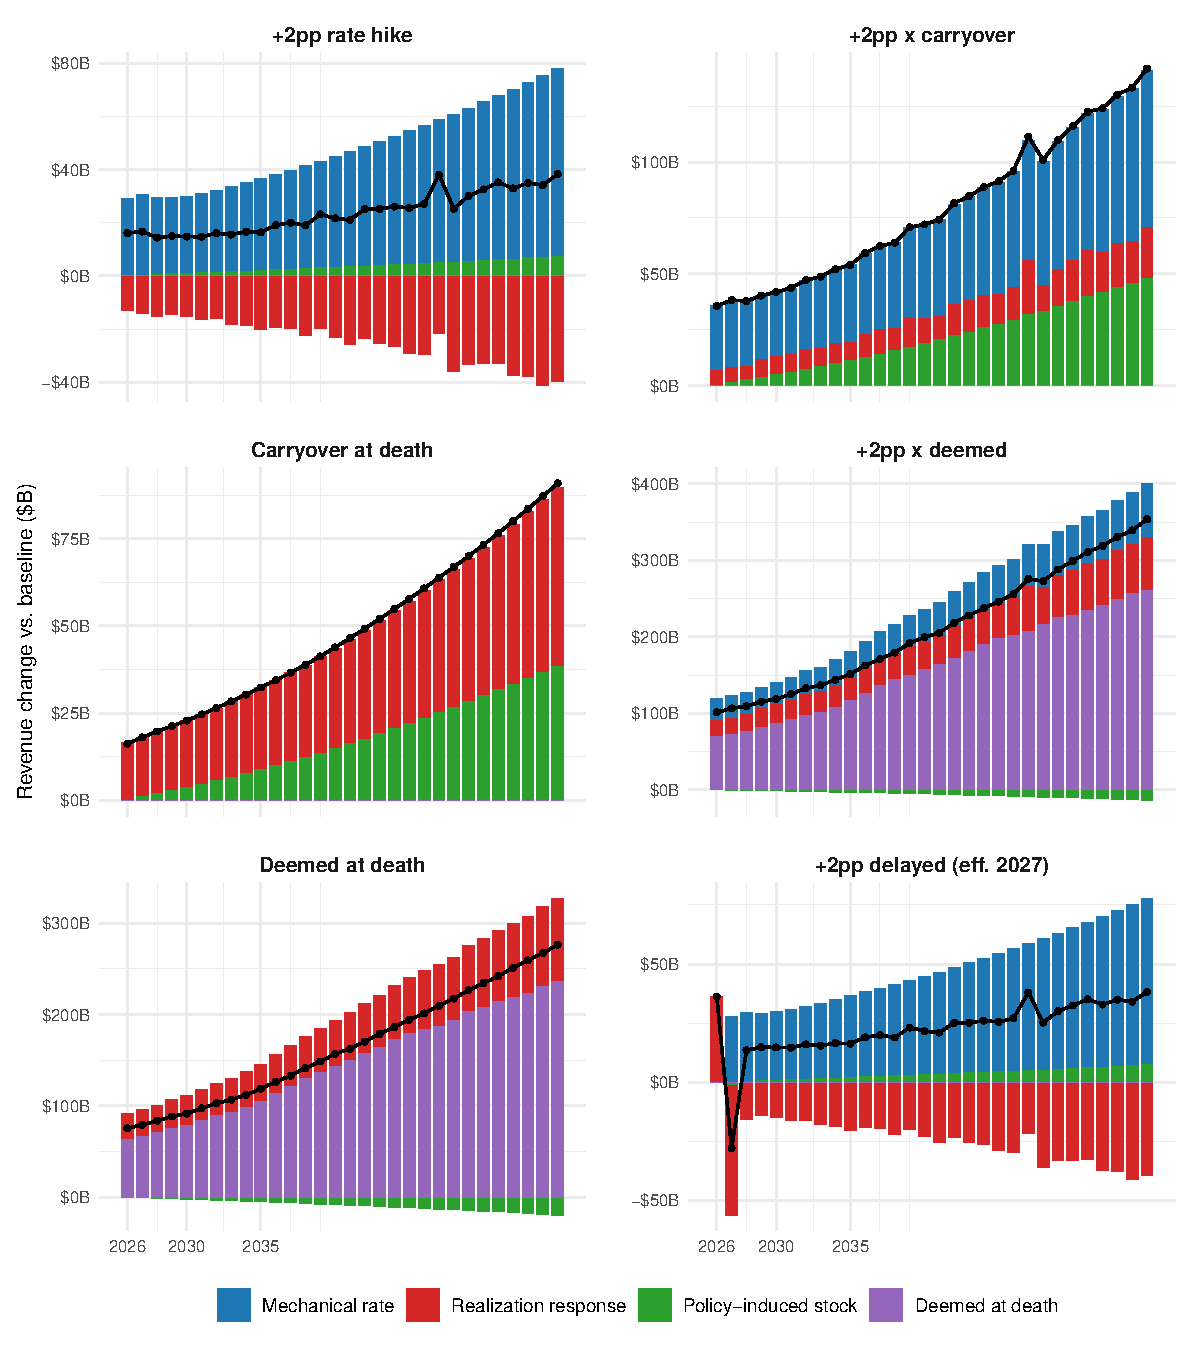
\includegraphics[width=\linewidth]{figures/decomp_panel.pdf}%
}{%
  \fbox{\parbox[c][3in][c]{0.95\linewidth}{\centering\itshape
    [placeholder: 2$\times$3 decomposition panel.\\
     Generate via \texttt{Rscript build\_decomp\_panel.R <vintage>}.]}}%
}
\caption{Year-by-year revenue decomposition for the six reforms. Stacked
         bars are the cell-level channel attribution; the black line is
         the engine's conventional $\Delta R$ from the microdata pass.
         The bars sum to within $\sim$1\% of the engine line; the small
         gap is from bracket / NIIT / AMT non-linearities the cell algebra
         can't see.}
\label{fig:decomp}
\end{figure}

%===============================================================================
\appendix
%===============================================================================

\section{Notation}
\label{app:notation}

\begin{tabular}{ll}
\toprule
$a, t$                     & age cell, simulation year                              \\
$j \in \{B, S\}$           & baseline / scenario environment                        \\
$G^j_{a,t}$                & unrealized-gain dollar stock                           \\
$R^j_{a,t}$                & realized positive long-term gains                      \\
$r^j_{a,t} = R^j/G^j$      & total cell realization rate                            \\
$r^D_{a,t}$                & ordinary (Bellman-controlled) discretionary rate       \\
$\phi_I,\ \phi_P$          & fixed share, planned share of realizations             \\
$\tau^j_{a,t}$             & average long-term-gains marginal tax rate              \\
$m_{a,t}$                  & gain-weighted cell mortality                           \\
$\beta_t$                  & year-varying real-rate discount factor                 \\
$W^j_{a,t}$                & per-dollar Bellman value                               \\
$\kappa_{a,t}$             & per-dollar nontax-benefit intercept                    \\
$\psi$                     & global curvature parameter                             \\
$c_\phi^j(a,t)$            & holder-internalized death-stock burden share           \\
$\theta$                   & heir-burden internalization weight (carryover)         \\
$F^j_{a,t}=(1-c_\phi^j)\tau^j$ & death-state forgiveness value                      \\
$\Delta G_{a,t}$           & policy-induced gain-stock divergence                   \\
$\omega_{a\to h}$          & SCF-derived dollar-weighted heir-age distribution      \\
$A_{a\to h}$               & age-aging operator (one-year increment)                \\
\bottomrule
\end{tabular}

\section{Bellman}
\label{app:bellman}

\subsection{Modeling closure}

Tax-Simulator is a repeated cross-section, so \dyn\ can't maintain
record-level dynamic wealth histories. The natural dynamic unit is the
representative age-year cell, treated as a synthetic cohort. The Bellman
is normalized to one dollar of unrealized gain in cell $(a, t)$; the
bathtub then scales chosen realization rates by the cell's actual dollar
stock. Baseline gain-stock growth is treated as an additive exogenous
inflow that cancels in the $\Delta G$ recurrence between scenario and
baseline (Appendix~\ref{app:bathtub}). The model is partial equilibrium:
tax payments are absorbed by an unmodeled outside margin (lower
consumption, lower other saving, borrowing, or higher labor supply); the
discount factor $\beta$ prices that outside-margin timing cost. Asset
allocation, portfolio returns, and dynastic heir choices are out of scope.

\subsection{Primitives}

For each cell the baseline pipeline supplies $\GB_{a,t}, \RB_{a,t},
\rB_{a,t}, m_{a,t}, \tauB_{a,t}$; scenario rates $\tauS_{a,t}$ and a
per-asset death-regime vector come from the policy YAML. The discount
factor series $\{\beta_t\}$ is constructed by Fisher-deflating the
ten-year-Treasury yield $\texttt{tsy\_10y}$ by year-$t$ YoY CPI-U from
Macro-Projections (the user memo \texttt{feedback\_kg\_dynamics\_real\_rates}
documents the decision to use a real discount factor). Mortality $m_{a,t}$
is gain-stock-weighted at the cell level:
$m_{a,t} = \sum_i w_i\,m^{\text{hh}}_i\,G^{\text{unit}}_i \big/
          \sum_i w_i\,G^{\text{unit}}_i$,
where $m^{\text{hh}}_i$ is per-household ($q^{\text{death}}_1 q^{\text{death}}_2$
for joint filers, $q^{\text{death}}_1$ otherwise). This corrects a known
bias in earlier specs that taxpayer-weighted mortality overstated $m$ by
$2$--$3\times$ relative to the per-dollar mortality the Bellman should use.

The age grid is extended past the bathtub topcode (age 80) to 119 using an
SSA Trustees life table (Alternative 2, 50/50 male/female blend), with
$r^B(a) = r^B(80)$ held flat in the tail so the continuation value of an
80-year-old is anchored to the empirical topcode-pool realization rate rather
than the model-internal zero.

\subsection{Equation and FOC}

The Bellman~(\ref{eq:bellman}) prices, per dollar of unrealized gain in
$(a,t)$:
\begin{itemize}
  \item the nontax benefit of realizing now,
        $b(r^D; \kappa, \psi) = \kappa r^D - (\psi/2)(r^D)^2$;
  \item the contemporaneous tax cost $-\tau^j r^D$;
  \item the discounted continuation value of dollars that survive and remain
        unrealized,
        $(1 - r_{\text{exog}} - r^D)\,\beta(1-m)\,W^j_{a+1,t+1}$;
  \item the discounted death-state forgiveness value,
        $(1 - r_{\text{exog}} - r^D)\,\beta\,m\,F^j$.
\end{itemize}
The quadratic benefit is not mandatory but is the transparent first
prototype: $\kappa$ shifts the level of baseline realization motives,
$\psi$ controls response curvature, and the interior FOC~(\ref{eq:foc}) is
closed-form. At corner cells with $r^{D,B} = 0$ the inversion sets
$\kappa = MC^B$ exactly so the cell sits at the lower corner under
baseline.

\subsection{Why the prior log-utility Bellman was discarded}

An earlier version of this model used a per-dollar log-benefit Bellman
with an exponential response rule
$r^{D,S} = r^{D,B}\exp\{-\eta(P^S - P^B)\}$, where $P^j$ is a tax-price
wedge constructed from $W^j$. The trouble is that once the cell intercept
$\kappa$ is recovered from the baseline FOC, the implied response is
insensitive to $\eta$ --- it cancels out of $r^S/r^B$. The
quadratic-direct-control formulation in~(\ref{eq:bellman}) sidesteps this
by keeping the level parameter ($\kappa$) and the curvature parameter
($\psi$) algebraically separate.

\section{Three-bucket realization timing}
\label{app:buckets}

\subsection{Bucket shares}

Total cell realizations are partitioned by~(\ref{eq:buckets}). The fixed
share $\phi_I = 0.40$ is held outside the Bellman's choice set and outside
the planned-timing channel. The planned share $\phi_P$ is calibrated jointly
with $\psi$ against the short-run target (Appendix~\ref{app:calib}); its
production value is $0.3041$. The ordinary Bellman bucket therefore controls
$(1 - \phi_I - \phi_P)\,\rB \approx 0.296\,\rB$ of baseline realizations.
The upper bound on the Bellman control is
$r_{\text{exog},B} = (\phi_I + \phi_P)\,\rB$.

\subsection{Planned-timing mechanics}

For each cell and year $t$, a fraction
$\xi_{t,t'} = \mathrm{clip}\!\left(\frac{\tauS_{t} - \tauS_{t'}}{w_{\text{ref}}},
                                   0,\, 1\right)$
of the planned-bucket dollars in year $t$ is shifted to a nearby year
$t' \in \{t-1, t, t+1\}$ (timing window $= 1$), where $w_{\text{ref}} = 0.05$
is the reference wedge: a $5$pp tax differential moves the full bucket; a
$1$pp differential moves $20\%$. Dollars are conserved: shifts sum to zero
across the window. The planned bucket has no permanent effect on aggregate
realizations and produces clean pull-back/payback patterns under temporary
shocks and announcement-effective splits.

\subsection{Identification}

The two calibration moments are orthogonal in the limit of a small
permanent-only shock: $\phi_P$ is silent on the long-run response (planned
dollars retime within a window but do not change the long-run flow) and
$\psi$ is silent on the announcement-year response in the limit of zero
$\phi_P$. Nested bisection (outer: $\phi_P$; inner: $\psi$) converges in
$\sim$10--20 outer $\times$ 5--10 inner iterations.

\section{Death channels}
\label{app:death}

\subsection{Forgiveness value $F$ and the regime triplet}

At death, the holder values the cell at $F^j = (1 - c_\phi^j)\,\tau^j$,
where $c_\phi^j \in [0, 1]$ is the burden share the current holder
internalizes on dollars whose realization is being decided today. Three
canonical regimes:
\begin{equation}
F = \begin{cases}
  \tau,             & \text{step-up}     \quad (c_\phi = 0)        \\
  (1-\theta)\tau,   & \text{carryover}   \quad (c_\phi = \theta)   \\
  0,                & \text{deemed}      \quad (c_\phi = 1).
\end{cases}
\end{equation}
Under step-up, death extinguishes liability for the current holder, so
holding gains into death is worth the full $\tau$. Under deemed
realization, no liability is forgiven and the death option has zero
value. Carryover sits between: liability isn't extinguished at the
family level, but the current holder may not fully internalize the
heir's future tax burden. The parameter $\theta \in [0, 1]$ governs that
internalization; $\theta = 1$ makes carryover look like deemed to the
holder; $\theta = 0$ makes it look like step-up. Production default is
$\theta = 0.5$, reported as a sensitivity since the empirical literature
doesn't pin it down sharply. Note that $F$ is the \emph{holder's}
reduced-form valuation; physical stock routing is a separate object that
lives in the bathtub (Appendix~\ref{app:bathtub}).

\subsection{Per-asset regime triplet}

Five wealth classes are tracked separately: equities, pass-throughs,
primary home, other (non-primary) home, and real-estate funds. The policy
YAML carries one regime code per asset class:
\begin{equation*}
\text{regime code}_k =
  \begin{cases} 0 & \text{step-up}\\ 1 & \text{carryover}\\ 2 & \text{deemed}\end{cases}
\end{equation*}
At each cell, the per-asset codes are resolved to a triplet
$(\delta_{\text{vanish}}, \delta_{\text{route}}, \delta_{\text{realize}})$
by gain-stock-weighted averaging:
\begin{equation}
\delta_{\bullet}(a, t) = \frac{\sum_{k} \GB_{k,a,t}\,\mathbf{1}\{\text{code}_k = \bullet\}}
                              {\sum_{k} \GB_{k,a,t}},
\quad \bullet \in \{\text{step-up, carryover, deemed}\}.
\end{equation}
These shares feed the bathtub recurrence (route $\to$ heir routing, realize
$\to$ deemed-at-death revenue, vanish $\to$ step-up). The holder-side
$c_\phi(a,t)$ in the Bellman is
$c_\phi = \theta\,\delta_{\text{route}} + 1\cdot\delta_{\text{realize}}
        + 0 \cdot \delta_{\text{vanish}}$, with one additional adjustment
on primary-home gains under deemed: see~\ref{app:121} below.

\subsection{\S{121} carve-out on primary-home gains}
\label{app:121}

Under deemed realization, primary-home gains are taxed at death net of the
\S{121} exclusion (\$250k single, \$500k joint). The per-record taxable
primary-home gain is
\begin{equation}
g^{\text{pri,121}}_{i} = \max\!\left(0,\; g^{\text{pri}}_{i}
                                     - \texttt{pref.kg\_sec121\_excl}_{i}\right),
\end{equation}
and the cell-level adjustment to the deemed-channel base is the
gain-stock-weighted utilization ratio
$\rho^{121}(a,t) = G^B_{\text{pri,121}}(a,t) / G^B_{\text{pri}}(a,t)$,
applied within the regime mix on the primary-home asset class. \S{121}
applies only to deemed; under carryover the basis carries to heirs with
their own future eligibility, and under step-up the exclusion is moot.

\subsection{Terminal-charity model}
\label{app:charity}

Bequests directed to qualifying charities are deductible from the estate
and avoid the deemed-realization tax base. We model the share of decedent
gain stock that is routed to charitable bequests as a two-stage logistic
function of the decedent's 2026-real estate value
$E_{i, 2026} = E_i \cdot \mathrm{CPI\text{-}U}_{2026} / \mathrm{CPI\text{-}U}_{t}$
(in millions):
\begin{align}
p^{\text{ext}}_i  &= \sigma(\alpha_{\text{ext}}
                          + \beta_{\text{ext}}\log E_{i, 2026}),
                          & (\alpha_{\text{ext}}, \beta_{\text{ext}}) &= (-2.415, 0.458),\\
p^{\text{int}}_i  &= \sigma(\alpha_{\text{int}}
                          + \beta_{\text{int}}\log E_{i, 2026}),
                          & (\alpha_{\text{int}}, \beta_{\text{int}}) &= (-1.872, 0.468),\\
p^{\text{char}}_i &= p^{\text{ext}}_i \cdot p^{\text{int}}_i,
\end{align}
where $\sigma(\cdot)$ is the logistic CDF, $p^{\text{ext}}$ is the
probability of any charitable bequest, and $p^{\text{int}}$ scales the
dollar share conditional on participation. Cell-level
$\overline{p^{\text{char}}}(a,t)$ is dollar-of-gain-weighted; the deemed
channel multiplies the cell's decedent stock by
$(1 - \overline{p^{\text{char}}})$ before computing taxable death revenue.
Logistic coefficients are calibrated to IRS-SOI estate-tax data on the
share of estates making charitable bequests and the share of those bequest
dollars relative to gross estate.

\subsection{SCF-derived heir distribution}

Under carryover, decedent gain stock routes to heir cells through an age
operator $\omega_{a \to h}$. Earlier specs used a Gaussian placeholder
($h \sim N(a - 30, 5^2)$); the production specification uses
\texttt{resources/heir\_distribution\_scf2022.csv}, a dollar-weighted
heir-age distribution constructed from the 2022 Survey of Consumer Finances
inheritance records. The build script (\texttt{build\_heir\_distribution.R})
filters non-gift transfers, applies the Gale-Sabelhaus 2024 recency-of-receipt
weights to convert the stock of past inheritances into a current-year flow,
and dollar-weights heir ages. The resulting $\omega$ has heavier mass on
ages 55--70 than the Gaussian placeholder, reflecting that high-wealth
decedents are themselves older and route to relatively older heirs.

\section{Bathtub recurrence}
\label{app:bathtub}

\subsection{State}

The bathtub tracks $\Delta G_{a,t} = G^S_{a,t} - G^B_{a,t}$ on the cohort
grid $a \in [18, 80]$. The recurrence~(\ref{eq:bathtub}) has two channels:

\paragraph{Survivor channel.}
$\sum_a A_{a \to h}\,(1 - m^{\text{eff}}_{a,t})
   \left[(1 - r^S_{a,t})\,\Delta G_{a,t}
         + G^B_{a,t}\,(r^B_{a,t} - r^S_{a,t})\right]$.
The bracket's first term carries the previous-period $\Delta G$ forward net
of survivor-realization; the second term is the new $\Delta G$ generated
this period by the scenario realization-rate gap on the baseline stock.
$A_{a \to h}$ is a one-year aging operator.

\paragraph{Heir-routing channel.}
$\delta_{\text{route}}(a, t)\,\sum_a \omega_{a \to h}\,m^{\text{eff}}_{a,t}
   \,(G^B_{a,t} + \Delta G_{a,t})$.
Active only on the carryover share; routes the full decedent stock (baseline
$+$ deviation) through the SCF heir distribution to heir cells, where it
joins the survivor channel in the subsequent period.

The effective cell mortality $m^{\text{eff}}_{a,t}$ in the bathtub is the
same gain-stock-weighted quantity used in the Bellman.

\subsection{Lock-in clamp}

The cell-level revenue accounting includes a term
$\tau^S\,r^S\,\Delta G$ that captures revenue on the policy-induced stock.
Under permanent rate hikes $\Delta G$ can run sufficiently negative that
$r^S\,\Delta G$ would subtract more from the realization base than the cell
holds. The implementation clamps
\begin{equation}
\Delta G^{\text{eff}}_{a,t} = \max\!\left(\Delta G_{a,t},\, -G^B_{a,t}\right),
\label{eq:clamp}
\end{equation}
so cell-level drawdowns cannot exceed full depletion of the baseline gain
stock. The deemed-channel multiplier
$\mathrm{deemed\_factor}(a,t) = \max(0, (G^B + \Delta G)/G^B)$ has the same
non-negativity guarantee. The clamp matters only in extreme persistent-shock
cohorts; in production scenarios it binds rarely.

\subsection{Why an exogenous inflow can be omitted}

Baseline gain-stock evolution carries an additive exogenous inflow
(appreciation, new saving, portfolio-composition changes, imputation
residual). For the baseline-to-scenario delta the bathtub actually
tracks, that inflow cancels: if
$G^j_{t+1} = H^j(G^j_t, r^j_t) + I_{t+1}$ for $j \in \{B, S\}$ with a
common exogenous $I_{t+1}$, then
$\Delta G_{t+1} = H^S(G^S_t, r^S_t) - H^B(G^B_t, r^B_t)$, and $I_{t+1}$
drops out. So the bathtub never has to compute the inflow, and the
Bellman's FOC is unaffected by it (it's not caused by today's marginal
realization decision).

\section{Calibration procedure}
\label{app:calib}

\subsection{Cell intercept recovery (inner $\kappa$ inversion)}

For each candidate $\psi$, the baseline Bellman runs backward over $(a, t)$.
At each cell:
\begin{enumerate}
  \item Compute continuation value $W^B_{a+1, t+1}$ (already solved).
  \item Compute baseline marginal cost
        $MC^B_{a,t} = \tau^B + \beta(1-m)\,W^B_{a+1,t+1} + \beta\,m\,F^B$.
  \item Set $\kappa_{a,t} = MC^B_{a,t} + \psi\,r^{D,B}_{a,t}$, where
        $r^{D,B} = \rB - r_{\text{exog},B}$. At corner cells with
        $r^{D,B} = 0$ set $\kappa = MC^B$.
  \item Compute $W^B_{a, t}$ at the observed choice.
\end{enumerate}
This is analogous to recovering cell fixed effects.

\subsection{$\psi$ bisection against the long-run target}

For each candidate $\psi$ and recovered $\{\kappa\}$, solve the scenario
Bellman under a uniform $+1$pp perturbation, run the bathtub, and aggregate
to a model semi-elasticity at simulation year $30$:
\begin{equation}
\widehat{\epsilon}^{\text{LR}}(\psi) = \frac{\log R^S_{30} - \log R^B_{30}}{0.01}.
\end{equation}
Bisect $\psi$ until $\widehat{\epsilon}^{\text{LR}}(\psi) = -2.52$. The
anchor at year 30 is deliberately past the bathtub's $\sim$10-year stock
build-up so the calibration locks the long-run steady state rather than a
transient.

\subsection{$\phi_P$ bisection against the short-run target}

For each candidate $\phi_P$, re-solve the inner $\psi$ bisection (so the
long-run target stays satisfied), then run a delayed $+5$pp shock
(announced at $t$, effective at $t+1$) and compute the year-1
semi-elasticity:
\begin{equation}
\widehat{\epsilon}^{\text{SR}}(\phi_P) = \frac{\log R^S_{1} - \log R^B_{1}}{0.05}.
\end{equation}
Bisect $\phi_P$ until $\widehat{\epsilon}^{\text{SR}}(\phi_P) = +5.04$. The
outer bisection converges in $\sim$10--20 iterations; warm-starting the
inner $\psi$ search from the previous outer iteration's solution keeps the
total cost under an hour on a full-sample baseline.

\subsection{Re-calibration triggers}

Re-run the calibration whenever any of the following change: Tax-Data
vintage, the discount factor series ($\beta_t$), bucket shares
$(\phi_I, w_{\text{ref}}, \text{timing window})$, the death-regime parameter
$\theta$, mortality input, the SCF heir distribution, or any Bellman
primitive.

\section{Implementation notes}
\label{app:impl}

\subsection{Two-pass solve}

For each scenario, the bathtub pre-pass~(\texttt{kg\_dyn\_run\_bathtub\_pass})
performs:
\begin{enumerate}
  \item \textbf{Pass 1} (baseline) over the extended grid $[18, 119]$:
        recover $\kappa(a, t)$ and $W^B(a, t)$ from observed baseline
        realizations.
  \item Per-year scenario regime mix
        (\texttt{kg\_dyn\_build\_regime\_mix}): resolve per-asset codes to
        $(\delta_{\text{vanish}}, \delta_{\text{route}}, \delta_{\text{realize}})$,
        compute $c_\phi$, build the cell-level \S{121} adjustment.
  \item \textbf{Pass 2} (scenario): solve the Bellman using fixed
        $\{\kappa\}$ and $\psi$ to obtain $r^{D,S}(a, t)$.
  \item Planned-timing schedule from
        $\tauS - \tauB$ (\texttt{kg\_dyn\_build\_planned\_timing}).
  \item Per-year: combine buckets into $\rS_{a,t}$, run the bathtub step
        (\texttt{kg\_dyn\_step\_recurrence}), build the cell-level state
        table, persist to disk.
\end{enumerate}
The downstream behavior module
(\texttt{config/scenarios/behavior/kg\_dynamics/turnover.R}) is a pure
allocator: for each tax-unit record in year $t$, it reads the year's
state table and translates cell quantities to per-record \texttt{kg\_lt}
adjustments via \texttt{kg\_dyn\_apply\_to\_records}.

\subsection{Resources}

\begin{itemize}
  \item \texttt{resources/PerLifeTables\_\{M,F\}\_Alt2\_TR2024.csv}:
        SSA Trustees Report Alt-2 life table for the 81--119 Bellman tail.
  \item \texttt{resources/heir\_distribution\_scf2022.csv}: SCF-2022
        dollar-weighted heir-age distribution.
\end{itemize}

\subsection{Out of scope}

\dyn\ does not currently model: (a) per-asset-class $\psi$ heterogeneity,
(b) age-varying $\psi$, (c) an embedded-gain-ratio cell-state dimension,
(d) record-level longitudinal wealth histories, or (e) dynastic heir
realization choices. Per-asset $\psi$ is the most likely near-term
extension; the asset-class infrastructure is already in place
(\texttt{KG\_DYN\_ASSET\_CLASSES}).

\end{document}
